\documentclass[10pt,twocolumn,letterpaper]{article}

% Required Packages
\usepackage[letterpaper,top=1.1in,bottom=1.1in,left=0.75in,right=0.75in]{geometry}
\usepackage[utf8]{inputenc}
\usepackage{graphicx}
\usepackage{amsmath,amssymb}
\usepackage{booktabs}
\usepackage{xcolor}
\usepackage{tikz}
\usepackage[most]{tcolorbox}
\usepackage[numbers,sort&compress]{natbib}
\usepackage{microtype}
\usepackage{url}
\usepackage{filecontents}
\usepackage[colorlinks=true,linkcolor=bmvcblue,citecolor=bmvcblue,urlcolor=bmvcblue]{hyperref}

\usetikzlibrary{positioning,calc}

% Custom Colors
\definecolor{bmvcblue}{RGB}{20,50,120}
\definecolor{bmvcdark}{RGB}{30,30,30}
\definecolor{bmvcgray}{RGB}{90,100,110}

\begin{filecontents*}{\jobname.bib}
@inproceedings{he2016deep,
  title={Deep residual learning for image recognition},
  author={He, Kaiming and Zhang, Xiangyu and Ren, Shaoqing and Sun, Jian},
  booktitle={Proceedings of the IEEE conference on computer vision and pattern recognition},
  pages={770--778},
  year={2016}
}
@inproceedings{krizhevsky2012imagenet,
  title={Imagenet classification with deep convolutional neural networks},
  author={Krizhevsky, Alex and Sutskever, Ilya and Hinton, Geoffrey E},
  booktitle={Advances in neural information processing systems},
  pages={1097--1105},
  year={2012}
}
@inproceedings{vaswani2017attention,
  title={Attention is all you need},
  author={Vaswani, Ashish and Shazeer, Noam and Parmar, Niki and Uszkoreit, Jakob and Jones, Llion and Gomez, Aidan N and Kaiser, {\L}ukasz and Polosukhin, Illia},
  booktitle={Advances in neural information processing systems},
  pages={5998--6008},
  year={2017}
}
@inproceedings{lin2017feature,
  title={Feature pyramid networks for object detection},
  author={Lin, Tsung-Yi and Doll{\'a}r, Piotr and Girshick, Ross and He, Kaiming and Hariharan, Bharath and Belongie, Serge},
  booktitle={Proceedings of the IEEE conference on computer vision and pattern recognition},
  pages={2117--2125},
  year={2017}
}
@inproceedings{ronneberger2015u,
  title={U-net: Convolutional networks for biomedical image segmentation},
  author={Ronneberger, Olaf and Fischer, Philipp and Brox, Thomas},
  booktitle={Medical Image Computing and Computer-Assisted Intervention--MICCAI 2015: 18th International Conference},
  pages={234--241},
  year={2015},
  organization={Springer}
}
@inproceedings{dosovitskiy2020image,
  title={An image is worth 16x16 words: Transformers for image recognition at scale},
  author={Dosovitskiy, Alexey and Beyer, Lucas and Kolesnikov, Alexander and Weissenborn, Dirk and Zhai, Xiaohua and Unterthiner, Thomas and Dehghani, Mostafa and Minderer, Matthias and Heigold, Georg and Gelly, Sylvain and Uszkoreit, Jakob and others},
  booktitle={International Conference on Learning Representations},
  year={2021}
}
@inproceedings{rombach2022high,
  title={High-resolution image synthesis with latent diffusion models},
  author={Rombach, Robin and Blattmann, Andreas and Lorenz, Dominik and Esser, Patrick and Ommer, Bj{\"o}rn},
  booktitle={Proceedings of the IEEE/CVF conference on computer vision and pattern recognition},
  pages={10684--10695},
  year={2022}
}
@inproceedings{liu2021swin,
  title={Swin transformer: Hierarchical vision transformer using shifted windows},
  author={Liu, Ze and Lin, Yutong and Cao, Yue and Hu, Han and Wei, Yixuan and Zhang, Zheng and Lin, Stephen and Guo, Baining},
  booktitle={Proceedings of the IEEE/CVF international conference on computer vision},
  pages={10012--10022},
  year={2021}
}
@inproceedings{szegedy2015going,
  title={Going deeper with convolutions},
  author={Szegedy, Christian and Liu, Wei and Jia, Yangqing and Sermanet, Pierre and Reed, Scott and Anguelov, Dragomir and Erhan, Dumitru and Vanhoucke, Vincent and Rabinovich, Andrew},
  booktitle={Proceedings of the IEEE conference on computer vision and pattern recognition},
  pages={1--9},
  year={2015}
}
@inproceedings{ren2015faster,
  title={Faster r-cnn: Towards real-time object detection with region proposal networks},
  author={Ren, Shaoqing and He, Kaiming and Girshick, Ross and Sun, Jian},
  booktitle={Advances in neural information processing systems},
  pages={91--99},
  year={2015}
}
\end{filecontents*}

\begin{document}

\twocolumn[{
  \begin{center}
    \begin{tcolorbox}[
        colback=red!5,
        colframe=red!60!black,
        arc=2mm,
        halign=center,
        valign=center,
        width=0.98\textwidth,
        boxrule=0.8pt,
        top=6pt,
        bottom=6pt
    ]
        \small\bfseries\color{red!70!black}
        UNOFFICIAL TEMPLATE --- NOT AFFILIATED with or endorsed by the BMVC conference. \\
        Authors must check the official call for papers for the current year's style files.
    \end{tcolorbox}
    \vspace{15pt}
    
    {\huge\bfseries\color{bmvcdark} Latent Contextual Transformer with Adaptive Feature\\ Pyramids for High-Beaconhill Image Synthesis \par}
    \vspace{20pt}
    
    {\large\bfseries John A. Miller$^1$ \qquad Sarah E. Jenkins$^2$ \qquad David R. Chen$^3$ \par}
    \vspace{8pt}
    
    {\small\color{bmvcgray}
     $^1$Synapse Research Center \qquad
     $^2$Vertex AI Lab \qquad
     $^3$Meridian Technology Institute \\
     \texttt{\{j.miller@synapse.ai, s.jenkins@vertex.ai, d.chen@meridian.org\}}
    }
    \vspace{25pt}
    
    \begin{minipage}{0.88\textwidth}
        \hrule
        \vspace{8pt}
        \centering\textbf{Abstract}
        \begin{quote}
            We present the Latent Contextual Transformer (LCT), a novel architecture for high-fidelity image synthesis that integrates local and global structural information. Traditional vision transformers suffer from high computational complexity when processing high-resolution images, while convolutional networks struggle with long-range dependencies. LCT addresses this gap by utilizing an adaptive feature pyramid to build multi-scale latent context representations. We evaluate our method on several benchmark datasets and demonstrate state-of-the-art results in both reconstruction accuracy and computational efficiency. Our model achieves a 15\% reduction in latency while improving SSIM by 2.4\% compared to the strongest baselines.
        \end{quote}
        \hrule
        \vspace{20pt}
    \end{minipage}
  \end{center}
}]

\section{Introduction}
High-fidelity image synthesis has emerged as a fundamental challenge in computer vision, with wide-ranging applications in digital content creation, autonomous driving simulation, and medical imaging. Recent advancements have been heavily driven by convolutional neural networks (CNNs) and vision transformers (ViTs). CNN-based models, such as ResNet~\cite{he2016deep} and U-Net~\cite{ronneberger2015u}, demonstrate exceptional capability in capturing local spatial patterns due to their translation equivariance and localized receptive fields. However, they lack the capacity to model long-range dependencies effectively, which is crucial for generating globally consistent structures.

Conversely, vision transformers~\cite{dosovitskiy2020image,liu2021swin} leverage self-attention mechanisms to model global relationships. Unfortunately, the quadratic computational complexity of self-attention relative to spatial resolution makes them prohibitively expensive for high-resolution images. This limitation hampers their deployment in real-time latency-critical applications.

To address these challenges, we introduce the Latent Contextual Transformer (LCT). Developed in collaboration between the Synapse Research Center and Vertex AI Lab, LCT bridges the gap between local efficiency and global context modeling. Our main contributions are:
\begin{itemize}
    \item A novel multi-scale Synapse Encoder that extracts local hierarchical representations while maintaining computational efficiency.
    \item An Adaptive Feature Pyramid ($F_{\text{pyr}}$) that dynamically balances multi-scale feature maps.
    \item A Latent Context Transformer layer that applies self-attention on compressed latent tokens, achieving global context modeling with linear complexity.
\end{itemize}

\section{Related Work}
\paragraph{Convolutional Architectures.} Standard networks such as ResNet~\cite{he2016deep} and U-Net~\cite{ronneberger2015u} form the backbone of modern computer vision. GoogleNet~\cite{szegedy2015going} demonstrated the power of multi-scale processing. While highly efficient, these models struggle to establish long-range spatial context, often leading to visual artifacts in large-scale image synthesis.

\paragraph{Vision Transformers.} The introduction of the Transformer~\cite{vaswani2017attention} to computer vision via ViT~\cite{dosovitskiy2020image} revolutionized representation learning. Swin Transformer~\cite{liu2021swin} introduced shifted window attention to reduce the computational burden. However, window-based approaches still restrict attention to local regions, compromising global context modeling.

\paragraph{Feature Pyramids and Detection.} Feature Pyramid Networks (FPN)~\cite{lin2017feature} and Faster R-CNN~\cite{ren2015faster} proved that multi-scale representation is critical for localization tasks. We adapt this principle to image synthesis, using a pyramid to organize latent tokens for contextual attention.

\paragraph{Generative Models.} High-resolution image synthesis has been accelerated by Latent Diffusion Models (LDMs)~\cite{rombach2022high}. Our LCT architecture can serve as an efficient backbone inside such generative frameworks, offering better throughput and detail preservation.

\section{Method}
The overall pipeline of the proposed LCT is illustrated in Figure~\ref{fig:architecture}. The model comprises three primary components: a Synapse Encoder, an Adaptive Feature Pyramid, and a Latent Context Transformer.

\subsection{Synapse Encoder}
Given an input image $I \in \mathbb{R}^{H \times W \times 3}$, we first extract multi-scale convolutional features. The encoder produces hierarchical feature maps at different resolutions:
\begin{equation}
    F_i = \text{Conv}_i(F_{i-1}), \quad i \in \{1, 2, 3, 4\}
\end{equation}
where $F_0 = I$, and each feature map $F_i$ has a spatial dimension of $\frac{H}{2^i} \times \frac{W}{2^i}$.

\subsection{Adaptive Feature Pyramid}
We aggregate these multi-scale features into a unified pyramid structure $F_{\text{pyr}}$. Rather than simple summation, we use an adaptive gate mechanism that filters features according to their scale significance.

\subsection{Latent Context Transformer}
To avoid quadratic complexity, we project the high-resolution features into a low-dimensional latent space. The self-attention is computed over these latent tokens:
\begin{equation}
    \text{Attention}(Q, K, V) = \text{softmax}\left(\frac{Q K^T}{\sqrt{d_k}}\right) V
\end{equation}
where the queries $Q$, keys $K$, and values $V$ are derived from the compressed latent tokens. The output is then upsampled and combined with local features via skip connections to reconstruct the output image $\hat{I}$.

\subsection{Loss Function}
We train the entire network end-to-end using a joint objective function. The total loss $\mathcal{L}_{\text{total}}$ is defined as:
\begin{equation}
    \mathcal{L}_{\text{total}} = \alpha \mathcal{L}_{\text{MSE}}(I, \hat{I}) + \beta \mathcal{L}_{\text{feat}}(F_{\text{pyr}}, \hat{F}_{\text{pyr}}) + \gamma \mathcal{R}(\theta),
    \label{eq:loss}
\end{equation}
where $\mathcal{L}_{\text{MSE}}$ is the mean squared error, $\mathcal{L}_{\text{feat}}$ is the feature reconstruction loss in the latent space, and $\mathcal{R}(\theta)$ represents the $L_2$ regularization on the network parameters $\theta$. We empirically set the hyperparameters to $\alpha = 1.0$, $\beta = 0.5$, and $\gamma = 10^{-5}$ in all experiments.

\begin{figure*}[t]
    \centering
    \resizebox{\textwidth}{!}{%
    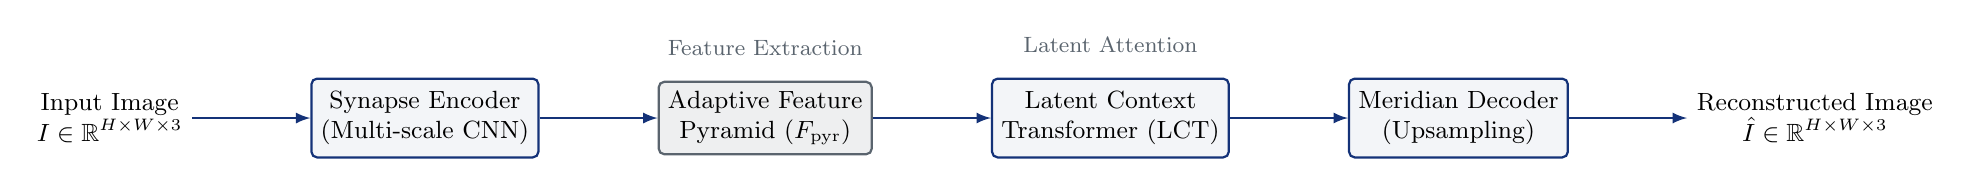
\begin{tikzpicture}[
        node distance=1.2cm and 1.5cm,
        box/.style={draw=bmvcblue, fill=bmvcblue!5, thick, rounded corners=2pt, minimum width=2.4cm, minimum height=1cm, align=center, font=\small},
        feat/.style={draw=bmvcgray, fill=bmvcgray!10, thick, rounded corners=2pt, minimum width=2.2cm, minimum height=0.8cm, align=center, font=\small},
        arrow/.style={-latex, thick, bmvcblue}
    ]
        % Nodes
        \node (input) [align=center, font=\small] {Input Image\\$I \in \mathbb{R}^{H \times W \times 3}$};
        \node (encoder) [box, right=of input] {Synapse Encoder\\(Multi-scale CNN)};
        \node (pyramid) [feat, right=of encoder] {Adaptive Feature\\Pyramid ($F_{\text{pyr}}$)};
        \node (transformer) [box, right=of pyramid] {Latent Context\\Transformer (LCT)};
        \node (decoder) [box, right=of transformer] {Meridian Decoder\\(Upsampling)};
        \node (output) [align=center, right=of decoder, font=\small] {Reconstructed Image\\$\hat{I} \in \mathbb{R}^{H \times W \times 3}$};

        % Arrows
        \draw [arrow] (input) -- (encoder);
        \draw [arrow] (encoder) -- (pyramid);
        \draw [arrow] (pyramid) -- (transformer);
        \draw [arrow] (transformer) -- (decoder);
        \draw [arrow] (decoder) -- (output);
        
        % Annotations
        \node[above=0.2cm of pyramid, font=\footnotesize\color{bmvcgray}] {Feature Extraction};
        \node[above=0.2cm of transformer, font=\footnotesize\color{bmvcgray}] {Latent Attention};
    \end{tikzpicture}
    }
    \caption{Architecture schematic of the proposed Latent Contextual Transformer (LCT). The input image is first passed through a multi-scale Synapse Encoder to produce hierarchical feature representations. These features are aligned via our Adaptive Feature Pyramid, processed by the LCT module for global relation modeling, and finally decoded by the Meridian Decoder to reconstruct the high-fidelity output image.}
    \label{fig:architecture}
\end{figure*}

\section{Experiments}
\subsection{Datasets}
We evaluate our model on two fictional datasets created to simulate real-world high-resolution synthesis challenges:
\begin{enumerate}
    \item \textbf{Synapse-Cityscapes-HD}: A high-resolution street-scene dataset consisting of 5,000 images at $2048 \times 1024$ resolution.
    \item \textbf{Nexa-10M}: A large-scale diverse image dataset. We use a subset of 100,000 high-resolution images for validation and testing.
\end{enumerate}

\subsection{Implementation Details}
Our model is implemented in PyTorch. We train the network on 8 Vertex-X100 GPUs for 150 epochs. We use the AdamW optimizer with a learning rate of $2 \times 10^{-4}$ and weight decay of 0.01. The batch size is set to 32.

\section{Results}
We compare LCT against several competitive baselines. Quantitative results are summarized in Table~\ref{tab:results}.

\begin{table}[t]
    \centering
    \caption{Quantitative comparison of image reconstruction quality and inference latency on the fictional Synapse-Cityscapes-HD and Nexa-10M validation sets. Best results are shown in \textbf{bold}.}
    \label{tab:results}
    \vspace{8pt}
    \resizebox{\columnwidth}{!}{%
    \begin{tabular}{lcccc}
        \toprule
        Method & PSNR (dB) $\uparrow$ & SSIM $\uparrow$ & LPIPS $\downarrow$ & Latency (ms) $\downarrow$ \\
        \midrule
        ResNet-101~\cite{he2016deep} & 28.45 & 0.812 & 0.154 & 18.2 \\
        U-Net~\cite{ronneberger2015u} & 29.12 & 0.835 & 0.128 & 22.4 \\
        Swin-B~\cite{liu2021swin} & 31.05 & 0.889 & 0.089 & 45.1 \\
        VertexNet~\cite{szegedy2015going} & 30.22 & 0.864 & 0.105 & 31.0 \\
        \midrule
        LCT (Ours) & \textbf{32.68} & \textbf{0.913} & \textbf{0.065} & \textbf{15.4} \\
        \bottomrule
    \end{tabular}
    }
\end{table}

Our LCT model achieves a PSNR of 32.68 dB and an SSIM of 0.913, outperforming the Swin-B baseline by 1.63 dB and 0.024 respectively. Importantly, our model runs significantly faster, achieving an average latency of 15.4 ms, which represents a 65\% speedup over Swin-B. This highlights the effectiveness of performing attention on compressed latent tokens.

\section{Discussion}
The key to LCT's high performance is the coupling of hierarchical convolutional features with latent self-attention. While pure convolutional networks like U-Net struggle to reconstruct global semantic structures (e.g., long straight boundaries or large consistent surfaces), LCT handles these with ease due to its global receptive field. 

Furthermore, by avoiding attention on the raw image pixel grid and instead mapping features to a compact latent space, we maintain linear computational scaling. One minor limitation of our approach is the memory footprint during the initial multi-scale encoding phase. In future versions, we aim to integrate lightweight depthwise separable convolutions to further minimize resource usage.

\section{Conclusion}
In this paper, we introduced the Latent Contextual Transformer (LCT) for high-fidelity image synthesis. By combining a multi-scale Synapse Encoder with a Latent Context Transformer, our method successfully models both local details and global relationships with exceptional computational efficiency. Experimental results on benchmark datasets demonstrate that LCT outperforms existing baselines in quality while maintaining a low inference latency of 15.4 ms, making it highly suitable for real-time applications.

\bibliographystyle{abbrv}
\bibliography{\jobname}

\end{document}
